\chapter{Objetivos y Metodología}
\label{cap:objetivos}

%Una vez presentado el contexto en el que se sitúa este proyecto, en este capítulo se fijan los objetivos y requisitos que debe seguir la solución. Para ello primero se describirá el problema y se explicará porqué es importante hacer el seguimiento de los objetos; a continuación se fijarán los objetivos y requisitos en función del problema y, por último, se expondrá la metodología seguida.

\section{Descripción del problema y requisitos}
\label{sec:descripciondelproblema}

La navegación en entornos dinámicos, como puede ser una casa o una institución pública, supone un gran reto que superar ya que las personas o las mascotas pueden acercarse o cruzarse delante del robot o podríamos encontrarnos objetos del mobiliario que han sido movidos de su posición original y se encuentran en nuestro camino. En este escenario el robot no debería nunca ni chocar ni perderse en el entorno y debe llegar al destino impuesto por la mejor ruta disponible.\\

Por ejemplo, si nuestro robot está yendo desde el salón a la cocina de nuestra casa pero en su camino habitual y más optimo se encuentra un mueble, el robot debe darse cuenta rápidamente, esquivarlo, proseguir con su camino y ademas recordarlo para que cuando volvamos al salón de vuelta podamos esquivarlo más fácilmente.Por otro lado en nuestra casa también habrá personas, estas personas se moverán casi constantemente por la estancia por lo que no será del todo correcto tenerlas en cuenta a la hora de planificar nuestra ruta para navegar de un sitio a otro de la casa pero si que será muy importante no chocar con ellas.\\

Para analizar el entorno del robot usaremos el sensor láser, este sensor destaca por su alta precisión y su corto tiempo de procesado.\\

%El sistema debe cumplir los siguientes requisitos:
%\begin{enumerate}
%\item \textbf{Posición y velocidad.} El sistema que se implemente deberá estimar la posición y velocidad de los objetos. Estas medidas deberán ir acompañadas de una incertidumbre que indique su fiabilidad.
%\item \textbf{Escalable.} Se debe poder seguir varios objetos al mismo tiempo, incluso si se trata de objetos homogéneos indistinguibles para el detector.
%\item \textbf{Tiempo real.} El algoritmo se ejecuta en tiempo real. Éste debe ser lo suficientemente eficiente como para poder ser ejecutado en un robot sin perjudicar al resto de las funcionalidades, y debe ser ligero computacionalmente.
%\item \textbf{General.} El algoritmo debe poder ser utilizado con cualquier tipo de detector que devuelva como mínimo la posición de un objeto en un instante determinado del tiempo.
%\item \textbf{Varias instancias.} Se podrán ejecutar varias instancias del algoritmo paralelamente. Cada una de las instancias debe ser independiente de la otra, ya que pueden ejecutarse a frecuencias distintas.
%\item \textbf{Objetos dinámicos vs estáticos.} La naturaleza de los objetos puede variar y ser tanto dinámica como estática. El algoritmo debe ser capaz de adaptarse a ambas situaciones.
%\item \textbf{Extensible.} Se diseñará el algoritmo de tal forma que sea fácil ampliar su funcionalidad.
%\item \textbf{Independiente de la plataforma.} Es importante que el núcleo del algoritmo sea independiente de la plataforma en la que se pruebe para facilitar su exportación a otras plataformas.
%\item \textbf{Precisión y Robustez.} El algoritmo debe mejorar la precisión y robustez de los datos proporcionados por el detector.
%\end{enumerate}

\section{Objetivo del proyecto}
\label{sec:objetivos}

Se quiere diseñar un algoritmo genere un mapa en tiempo real, el cual será usado por el nodo de navegación de ROS para navegar por un entorno doméstico, ya sea indicando una posición x,y en el mapa o indicándole una estancia a la que navegar. Este mapa se construirá a partir de la mezcla de 3 mapas, mapa estático, mapa de largo plazo y mapa de corto plazo.\\
%hablar del mapa semántico
En primera instancia el algoritmo se validará haciendo uso de un simulador en el que se representa una casa con varios tipos de muebles, ya que resulta más fácil de depurar un algoritmo en un entorno virtual, que en un entorno real. Posteriormente el algoritmo se probará en distintas recreaciones de escenarios reales ,y se harán las modificaciones oportunas para adaptarlo al entorno real, y por ultimo se llevará a la competición.\\

Para simplificar la resolución del problema se ha dividido el proyecto en varios subobjetivos:

\begin{enumerate}
\item Se usarán las herramientas por defecto que nos ofrece ROS para creare el mapa de corto plazo en referencia a las mediciones tomadas por el laser. En un primer paso solo añadiremos los diferentes objetos que percibamos.
\item Se ampliará el algoritmo anterior para poder añadir y eliminar objetos que aparezcan o desparezcan del entorno. 
\item Se desarrollará un algoritmo para mezclar los mapas entre sí y así generar tanto el mapa de largo plazo como el mapa que usaremos para la navegación.
\item Se creará un servidor de mapas dinámicos que se inicializará con los mapas estático y de largo plazo y que generará el mapa final mezclando de loa mapas de largo plazo y de corto plazo.
\item Se usará el mapa final como parámetro del paquete de navegación de ROS, \textit{move base}, y del paquete de localización de ROS \textit{amcl}.
\item Se generará y usará un mapa semántico, en el que cada nivel de gris se asocie con una etiqueta para después ordenar al robot que navegue a dichas etiquetas.
\end{enumerate}

\section{Metodología de desarrollo}
\label{sec:metodologiadedesarrollo}

En el desarrollo del sistema descrito, el modelo de ciclo de vida utilizado ha sido el modelo en espiral basado en prototipos. Este modelo permite desarrollar el proyecto de forma incremental, aumentando la complejidad progresivamente y haciendo posible la generación de prototipos funcionales. Este planteamiento permite obtener productos parciales al final de cada ciclo que pueden ser evaluados, ya sea total o parcialmente. Esto facilita la adaptación a los cambios en los requisitos, circunstancia muy común en los proyectos de investigación.\\

\begin{figure} [hbtp]
  \begin{center}
    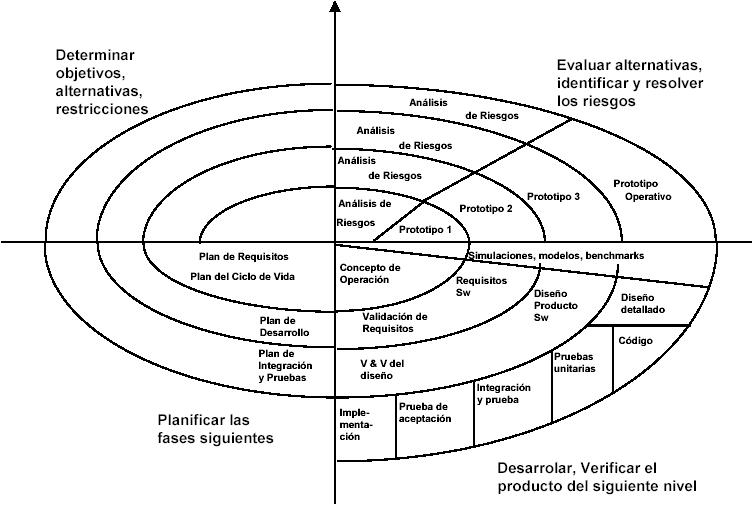
\includegraphics[width=16cm]{img/cap2/modelo_espiral}
  \end{center}
  \caption{Modelo en espiral.}
  \label{fig:modelo_espiral}
\end{figure}

El ciclo de vida de este modelo está dividido en ciclos. Cada ciclo representa una fase del proyecto y está dividido, a su vez, en 4 partes. Cada una de las partes tiene un objetivo distinto:

\begin{itemize}
\item \textbf{Determinar objetivos.} Se establecen las necesidades que debe cumplir el sistema en cada iteración teniendo en cuenta los objetivos finales. Según avanzan las iteraciones aumenta el coste del ciclo y su complejidad.
\item \textbf{Evaluar alternativas.} Se determinan diferentes formas de alcanzar los objetivos que se han establecido en la fase anterior. Se aborda el problema desde distintos puntos de vista, como, por ejemplo, el rendimiento del algoritmo en tiempo y espacio. Además, se consideran explícitamente los riesgos, intentando mitigarlos al máximo.
\item \textbf{Desarrollar y verificar.} Se desarrolla el producto siguiendo la mejor alternativa para poder alcanzar los objetivos del ciclo. Una vez diseñado e implementado el producto, se realizan las pruebas necesarias para comprobar su funcionamiento.
\item \textbf{Planificar.} Teniendo en cuenta los resultados de las pruebas realizadas, se planifica la siguiente iteración, se revisan los errores cometidos y se comienza un nuevo ciclo de la espiral.
\end{itemize}

\section{Plan de trabajo}
\label{sec:plandetrabajo}

Para poder abordar el problema se han marcado una serie de subobjetivos ha completar. Dichos hitos son los siguientes:

\begin{enumerate}
\item Estudio y comprensión de la composición de un mapa y como construirlo. Nos apoyaremos en las herramienta ofrecidas por ROS y que resultaran básicas para este fin, dicha herramientas son \textit{TF} \footnote{http://wiki.ros.org/tf} y \textit{Costmap}\footnotemark .
\footnotetext{http://wiki.ros.org/costmap\_2D}
\item Primer subobjetivo. Una vez conocido como funcionan los \textit{costmap} procederemos a crear un pequeño nodo en el que se cree un mapa con las observaciones instantáneas que percibimos con el láser.
\item Segundo subobjetivo. Extender el algoritmo anterior para poder añadir y eliminar objetos según entren o salgan de la escena.
\item Tercer subobjetivo. Modificar el paquete \textit{map\_server} para que acepte varios mapas como entrada y estudiar la manera de mezclar los mapas entre sí.
\item Fase de pruebas. Se le pasará al paquete de navegación de ROS, \textit{move\_base} ,el mapa resultante y se harán pruebas de navegación en el simulador y en el robot real.
\item Cuarto subobjetivo. Crear el mapa semántico, especificando las etiquetas naturales que tendrá una casa, salón, cocina, habitación... y usarlo para poder ir a la estancia que le indiquemos.
\end{enumerate}
